\subsection{YARN} \label{yarn}
Quando i dati hanno cominciato a diventare sempre più grandi, Hadoop File System è stato in grado di immagazzinarli, ma MapReduce è diventato un collo di bottiglia nelle prestazioni. Questo perché, in Hadoop 1.x, il JobTracker si occupava sia della gestione delle risorse, sia dell'elaborazione dei dati. Per questo motivo, in Hadoop 2.0\footnote{Hadoop 2.0 changelog: \href{https://hadoop.apache.org/release/2.2.0.html}{https://hadoop.apache.org/release/2.2.0.html}} è stato introdotto \textit{YARN\footnote{YARN docs: \href{https://hadoop.apache.org/docs/current/hadoop-yarn/hadoop-yarn-site/YARN.html}{https://hadoop.apache.org/docs/current/hadoop-yarn/hadoop-yarn-site/YARN.html}} (Yet Another Resources Navigator)} che separa il livello di gestione delle risorse dal livello di elaborazione. L'idea fondamentale di YARN è di dividere queste funzionalità in processi separati:
\begin{itemize}
    \item \textbf{ResourceManager}: è il processo master di YARN ed è responsabile dell'assegnazione e della gestione delle risorse tra tutte le applicazioni. Ogni volta che riceve una richiesta di elaborazione, la inoltra al gestore del nodo corrispondente (NodeManager) e alloca le risorse per il completamento della richiesta. Viene suddiviso in ulteriori due componenti:
    \begin{itemize}
        \item \textbf{Scheduler}: esegue la pianificazione in base all'applicazione assegnata e alle risorse disponibili. Non esegue altri compiti come il monitoraggio o il tracking e non garantisce un riavvio se un compito fallisce. 
        \item \textbf{ApplicationManager}: è responsabile di dell'accettazione dell'applicazione e della negoziazione del primo container\footnote{Per container si intende un insieme di risorse fisiche come RAM, core di CPU e disco su un singolo nodo.} dal gestore delle risorse. Riavvia anche il container ApplicationMaster se un job fallisce.
    \end{itemize}
    \item \textbf{NodeManager}: è l'agente del framework per ogni macchina ed è responsabile del monitoraggio del loro utilizzo delle risorse (cpu, memoria, disco, rete) e della segnalazione al ResourceManager. Si registra con il ResourceManager e invia \textit{heartbeat} (segnali) con lo stato di salute del nodo. Monitora l'uso delle risorse, esegue la gestione dei log e uccide anche un container in base alle indicazioni del gestore delle risorse. 
    \item \textbf{ApplicationMaster}: è una libreria specifica del framework e ha il compito di negoziare le risorse dal ResourceManager e lavorare con i NodeManager per eseguire e monitorare i job.
\end{itemize}

\begin{figure}[ht!]
    \centering
    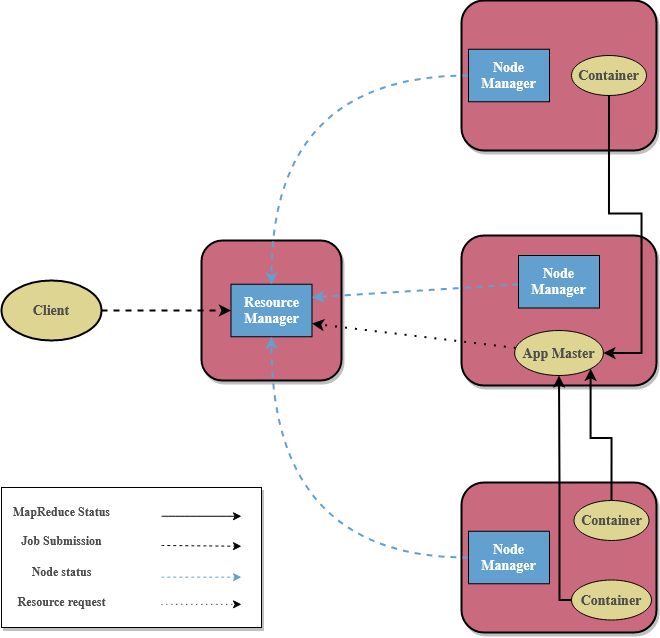
\includegraphics[width=0.8\textwidth]{img/yarn.png}
    \caption{Architettura YARN}
    \label{fig:yarn}
\end{figure}
\clearpage